\subsection*{Problema 34}

\textbf{Enunciado:} \\
Calcular la integral indefinida:
\begin{align*}
\int \dfrac{3x^4}{(x^2 + 1)^2} \, dx
\end{align*}

\textbf{Solución:} \\
Para resolver esta integral, podemos reescribir el numerador en términos de factores de $(x^2 + 1)$ para simplificar la fracción algebraica sin recurrir directamente a la sustitución trigonométrica.

Primero, expandimos el numerador manipulando algebraicamente $x^4$:
\begin{align*}
3x^4 &= 3(x^2 + 1 - 1)^2 \\
&= 3\left[(x^2 + 1)^2 - 2(x^2 + 1) + 1\right]
\end{align*}

Sustituimos esta expresión de vuelta en el integrando original:
\begin{align*}
&\int \dfrac{3x^4}{(x^2 + 1)^2} \, dx = \\
&\int \dfrac{3\left[(x^2 + 1)^2 - 2(x^2 + 1) + 1\right]}{(x^2 + 1)^2} \, dx
\end{align*}

dividimos cada término del numerador entre el denominador común $(x^2 + 1)^2$:
\begin{align*}
= 3 \int \left[ 1 - \dfrac{2}{x^2 + 1} + \dfrac{1}{(x^2 + 1)^2} \right] dx
\end{align*}

integramos término a término:
\begin{align*}
= 3 \int 1 \, dx &- 6 \int \dfrac{1}{x^2 + 1} \, dx \\
&+ 3 \int \dfrac{1}{(x^2 + 1)^2} \, dx
\end{align*}

Las primeras dos integrales son inmediatas:
\begin{align*}
3 \int 1 \, dx &= 3x \\
-6 \int \dfrac{1}{x^2 + 1} \, dx &= -6 \arctan(x)
\end{align*}

Para la tercera integral, $\int \dfrac{1}{(x^2 + 1)^2} \, dx$, utilizamos la sustitución trigonométrica $x = \tan(\theta)$, de donde $dx = \sec^2(\theta) \, d\theta$:
\begin{align*}
\int \dfrac{\sec^2(\theta)}{(\tan^2(\theta) + 1)^2} \, d\theta &= \int \dfrac{\sec^2(\theta)}{(\sec^2(\theta))^2} \, d\theta \\
&= \int \dfrac{1}{\sec^2(\theta)} \, d\theta \\
&= \int \cos^2(\theta) \, d\theta
\end{align*}

Usando la identidad del ángulo doble:
\begin{align*}
\int \dfrac{1 + \cos(2\theta)}{2} \, d\theta &= \dfrac{\theta}{2} + \dfrac{\sin(2\theta)}{4} \\
&= \dfrac{\theta}{2} + \dfrac{\sin(\theta)\cos(\theta)}{2}
\end{align*}

Regresando a la variable original $x$:
\begin{align*}
\theta &= \arctan(x), \\
\sin(\theta) &= \dfrac{x}{\sqrt{x^2 + 1}}, \quad \cos(\theta) = \dfrac{1}{\sqrt{x^2 + 1}}
\end{align*}

Por lo tanto, la tercera integral resulta en:
\begin{align*}
\dfrac{\arctan(x)}{2} + \dfrac{x}{2(x^2 + 1)}
\end{align*}

Multiplicando por el factor 3 externo:
\begin{align*}
3 \left( \dfrac{\arctan(x)}{2} + \dfrac{x}{2(x^2 + 1)} \right) = \dfrac{3}{2}\arctan(x) + \dfrac{3x}{2(x^2 + 1)}
\end{align*}

Agrupando todos los resultados parciales y añadiendo la constante de integración $C$:
\begin{align*}
3x &- 6\arctan(x) \\
&+ \dfrac{3}{2}\arctan(x) + \dfrac{3x}{2(x^2 + 1)} + C
\end{align*}

Simplificando los términos semejantes de $\arctan(x)$:
\begin{align*}
-6\arctan(x) + \dfrac{3}{2}\arctan(x) = -\dfrac{9}{2}\arctan(x)
\end{align*}

Finalmente, la solución general es:
\begin{align*}
3x - \dfrac{9}{2}\arctan(x) + \dfrac{3x}{2(x^2 + 1)} + C
\end{align*}

\begin{figure}[H]
	\centering
	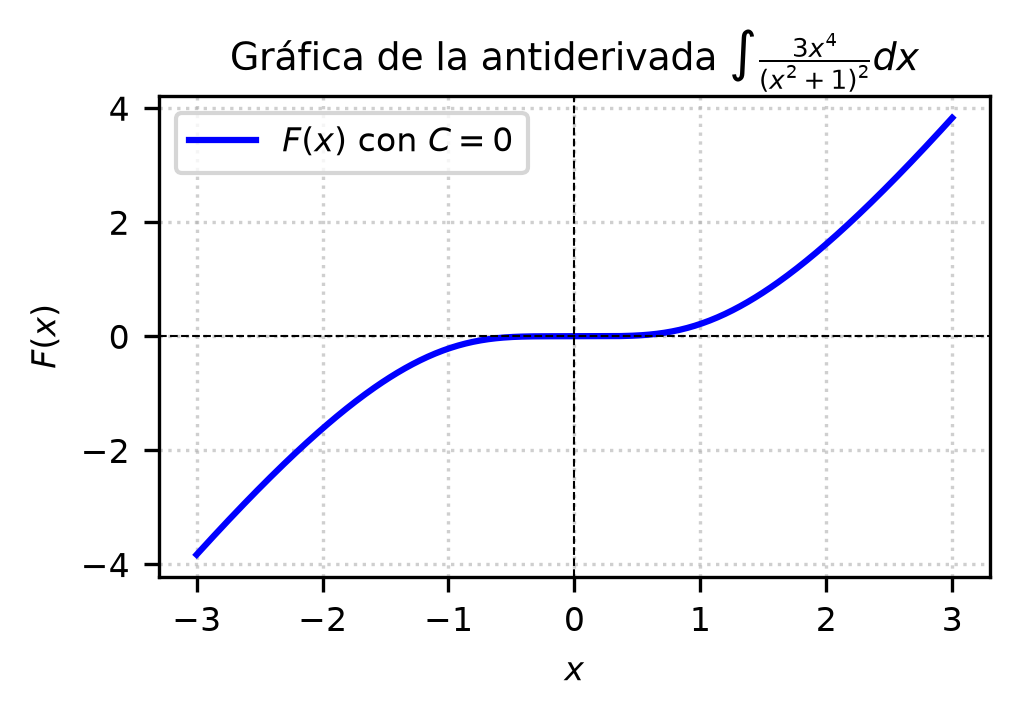
\includegraphics[width=\columnwidth]{semana_03/graficas/SEM03_P34_grafica.png}
	\caption{Representación gráfica de $f(x)$ y su antiderivada $F(x)$ evaluada para la constante de integración $C = 0$ (Problema 34).}
	\label{fig:problema34}
\end{figure}
